\documentclass[tikz,border=6pt]{standalone}
\usepackage{pgfplots}
\pgfplotsset{compat=1.18}
\usepgfplotslibrary{colormaps}
\usetikzlibrary{arrows, arrows.meta, calc}
\usetikzlibrary{decorations.markings}


\usepackage{amssymb,amsmath,mathtools}

\usepackage[T1]{fontenc}
\usepackage[utf8]{inputenc}
\usepackage{newpxtext,newpxmath}
\usepackage{sectsty}

\renewcommand{\Re}{\operatorname{\mathrm{Re}}}
\renewcommand{\Im}{\operatorname{\mathrm{Im}}}


\begin{document}
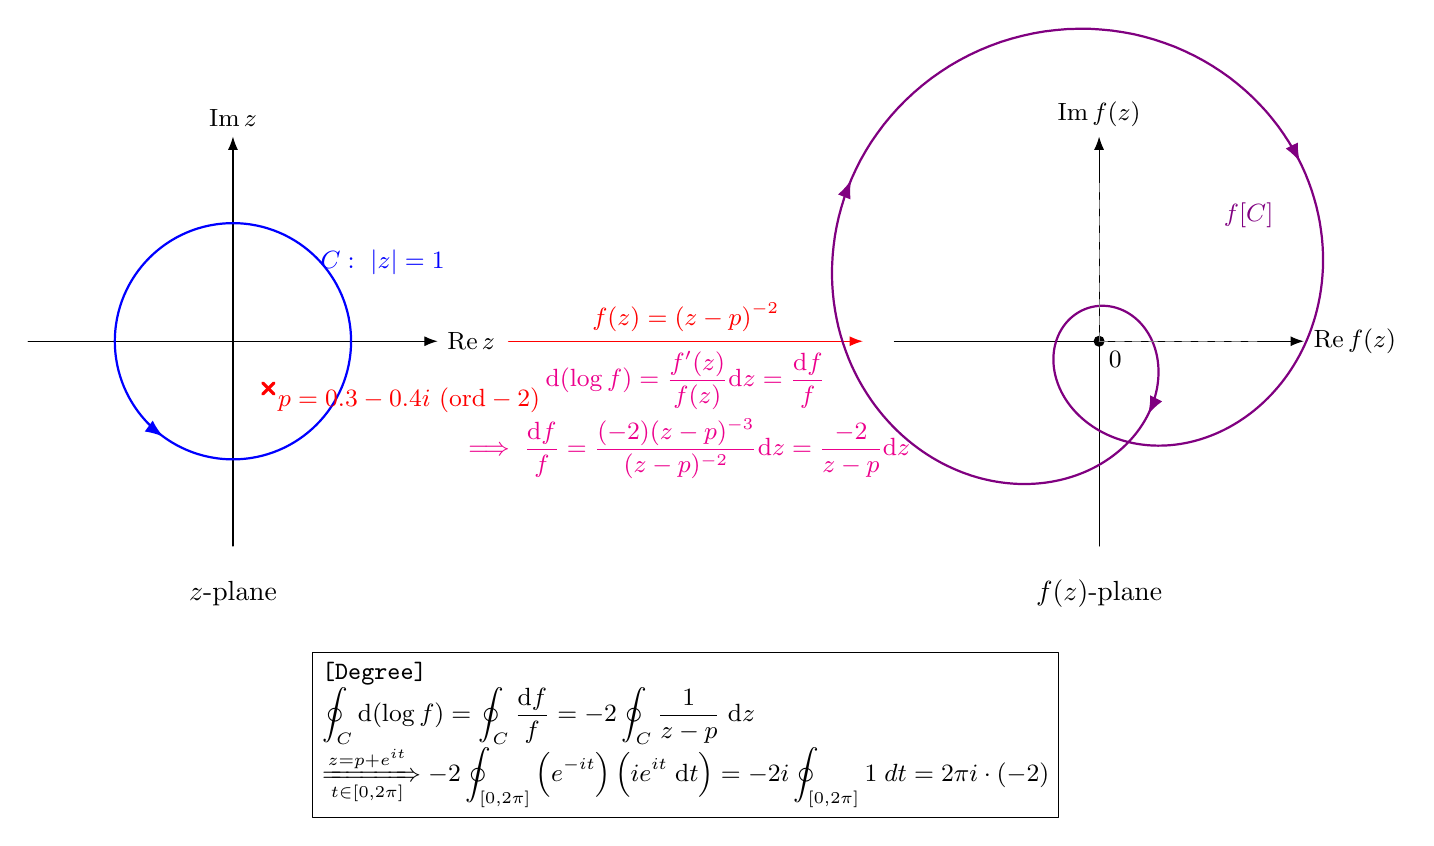
\begin{tikzpicture}[>=Latex, line cap=round, line join=round, font=\small]
%========================
% Left: z-plane
%========================
\begin{scope}[shift={(0,0)}]
	\node[font=\normalsize] at (0,-3.2) {$z$-plane};
	% axes
	\draw[->] (-2.6,0)--(2.6,0) node[right] {$\Re z$};
	\draw[->] (0,-2.6)--(0,2.6) node[above] {$\Im z$};
	% unit circle C (positively oriented) -- radius 1.5 for visibility
	\draw[blue,thick,postaction={decorate},
	decoration={markings, mark=at position 0.65 with {\arrow{>}}}]
	(0,0) circle (1.5);
	\node[blue] at (1.9,1.0) {$C:\ |z|=1$};
	
	% pole at p (order -2), choose concrete p inside C
	\draw[red,very thick] (0.45,-0.6) ++(-0.07,-0.07) -- ++(0.14,0.14);
	\draw[red,very thick] (0.45,-0.6) ++(-0.07,0.07)  -- ++(0.14,-0.14);
	\node[red, right] at (0.45,-0.75) {$p=0.3-0.4i$ ($\mathrm{ord} -2$)};
%	\node[red] at (-1.8,-1.7) {pole of order $-2$};
\end{scope}

% function label + order via winding form
% annotation: coefficients from Cauchy integral formula at z_0=p
\draw[->, red] (3.5,0) -- (8,0) node[midway, above, align=center] {$\displaystyle
	f(z)=(z-p)^{-2}$};
\draw[->, magenta, opacity=0] (3.5,0) -- (8,0) node[midway, below, align=center, opacity=1] {
	$\displaystyle\mathrm{d}(\log f)=\frac{f'(z)}{f(z)}\mathrm{d}z=\frac{\mathrm{d}f}{f}$\\ [2pt]
	$\displaystyle\implies\frac{\mathrm{d}f}{f}=\frac{(-2)(z-p)^{-3}}{(z-p)^{-2}}\mathrm{d}z=\frac{-2}{z-p}\mathrm{d}z$};

\node[draw=black, align=left] at (5.75,-5) {
	\texttt{[Degree]}\\
	$\displaystyle
	\oint_C \mathrm{d}(\log f)=\oint_C \frac{\mathrm{d}f}{f}=-2\oint_C \frac{1}{z-p}\; \mathrm{d}z$ \\
	$\displaystyle\xRightarrow[{t\in[0,2\pi]}]{z=p+e^{it}}-2\oint_{[0,2\pi]}\left(e^{-it}\right)\left(ie^{it}\; \mathrm{d}t\right)=-2i\oint_{[0,2\pi]}1\; dt=2\pi i\cdot (-2)$
};

%========================
% Right: f(z)-plane
%========================
\begin{scope}[shift={(11,0)}]
	\node[font=\normalsize] at (0,-3.2) {$f(z)$-plane};
	% axes
	\draw[->] (-2.6,0)--(2.6,0) node[right] {$\Re f(z)$};
	\draw[->] (0,-2.6)--(0,2.6) node[above] {$\Im f(z)$};
	
	% origin
	\fill (0,0) circle(2pt) node[below right] {$0$};
	
	% image curve f(C): z = 1.5 e^{it} -> w = 1/(z-p)^2
	% Let x = 1.5 cos t - 0.3,  y = 1.5 sin t + 0.4  (so z-p = x + i y).
	% Then (z-p)^2 = (x^2 - y^2) + i(2xy) and
	% 1/(z-p)^2 = [(x^2 - y^2) - i(2xy)] / [(x^2 + y^2)^2].
	\draw[violet,thick,
	postaction={decorate},
	decoration={markings,
			mark=at position 0.20 with {\arrow{>}},
			mark=at position 0.50 with {\arrow{>}},
			mark=at position 0.80 with {\arrow{>}}}]
	plot[domain=0:6.283, samples=700]
	({
			((1*cos(\x r)-0.3)^2 - (1*sin(\x r)+0.4)^2)
			/
			( ((1*cos(\x r)-0.3)^2 + (1*sin(\x r)+0.4)^2)^2 )
		},
	{
			-( 2*(1*cos(\x r)-0.3)*(1*sin(\x r)+0.4) )
			/
			( ((1*cos(\x r)-0.3)^2 + (1*sin(\x r)+0.4)^2)^2 )
		});
	\node[violet] at (1.9,1.6) {$f[C]$};
	
	% dashed rays to visualize winding (clockwise double)
	\draw[gray,dashed] (0,0) -- (2.1,0);
	\draw[gray,dashed] (0,0) -- (0,2.1);
\end{scope}

	
%	%========================
%	% Left: z-plane
%	%========================
%	\begin{scope}[shift={(0,0)}]
%		\node[font=\normalsize] at (0,3.2) {$z$-plane};
%		% axes
%		\draw[->] (-2.2,0)--(2.2,0) node[right] {$\Re z$};
%		\draw[->] (0,-2.2)--(0,2.2) node[above] {$\Im z$};
%		
%		% unit circle C (positively oriented) -- radius 1.5 for visibility
%		\draw[blue,thick,postaction={decorate},
%		decoration={markings, mark=at position 0.65 with {\arrow{>}}}]
%		(0,0) circle (1.5);
%		\node[blue] at (1.9,1.0) {$C:\ |z|=1$};
%		
%		% pole at p (order -2), choose concrete p inside C
%		\draw[red,very thick] (0.45,-0.6) ++(-0.07,-0.07) -- ++(0.14,0.14);
%		\draw[red,very thick] (0.45,-0.6) ++(-0.07,0.07)  -- ++(0.14,-0.14);
%		\node[red] at (0.95,-0.75) {$p=0.3-0.4i$};
%		\node[red] at (-1.8,-1.7) {pole of order $-2$};
%		
%		% function label + order via winding/logarithmic derivative
%		\node[align=left] at (0,-2.7) {$\displaystyle
%			f(z)=\frac{1}{(z-p)^{2}},\quad
%			\operatorname{ord}_{p} f
%			=\frac{1}{2\pi i}\!\oint_C \frac{df}{f}
%			=\frac{1}{2\pi i}\!\oint_C \frac{-2\,dz}{\,z-p\,}=-2.$};
%	\end{scope}
%	
%	%========================
%	% Right: w-plane = f(z)-plane
%	%========================
%	\begin{scope}[shift={(7.2,0)}]
%		\node[font=\normalsize] at (0,3.2) {$w=f(z)$-plane};
%		% axes
%		\draw[->] (-2.6,0)--(2.6,0) node[right] {$\Re w$};
%		\draw[->] (0,-2.6)--(0,2.6) node[above] {$\Im w$};
%		
%		% origin
%		\fill (0,0) circle(2pt) node[below right] {$0$};
%		
%		% image curve f(C): z = 1.5 e^{it} -> w = 1/(z-p)^2
%		% Let x = 1.5 cos t - 0.3,  y = 1.5 sin t + 0.4  (so z-p = x + i y).
%		% Then (z-p)^2 = (x^2 - y^2) + i(2xy) and
%		% 1/(z-p)^2 = [(x^2 - y^2) - i(2xy)] / [(x^2 + y^2)^2].
%		\draw[violet,thick,
%		postaction={decorate},
%		decoration={markings,
%			mark=at position 0.20 with {\arrow{>}},
%			mark=at position 0.50 with {\arrow{>}},
%			mark=at position 0.80 with {\arrow{>}}}]
%		plot[domain=0:6.283, samples=700]
%		({
%			((1.5*cos(\x r)-0.3)^2 - (1.5*sin(\x r)+0.4)^2)
%			/
%			( ((1.5*cos(\x r)-0.3)^2 + (1.5*sin(\x r)+0.4)^2)^2 )
%		},
%		{
%			-( 2*(1.5*cos(\x r)-0.3)*(1.5*sin(\x r)+0.4) )
%			/
%			( ((1.5*cos(\x r)-0.3)^2 + (1.5*sin(\x r)+0.4)^2)^2 )
%		});
%		\node[violet] at (1.9,1.6) {$f(C)$};
%		
%		% dashed rays to visualize winding (clockwise double)
%		\draw[gray,dashed] (0,0) -- (2.1,0);
%		\draw[gray,dashed] (0,0) -- (0,2.1);
%		
%		% annotation: Laurent coefficients via Cauchy integrals (about p)
%		\node[align=center] at (0,-2.45)
%		{$\displaystyle
%			f(z)=\frac{1}{(z-p)^{2}}
%			=\sum_{n=-\infty}^{\infty} c_n (z-p)^n,\qquad
%			c_n=\frac{1}{2\pi i}\!\oint_C \frac{f(\zeta)}{(\zeta-p)^{\,n+1}}\,d\zeta.$\\[4pt]
%			For $f(z)=1/(z-p)^{2}$:\quad
%			$c_{-2}=\frac{1}{2\pi i}\!\oint_C f(\zeta)\,(\zeta-p)\,d\zeta=1,\quad
%			c_n=0\ (n\neq -2).$\\[6pt]
%			$\mathrm{wind}\big(f(C),0\big)=-2
%			\ \Rightarrow\
%			\displaystyle \oint_C \frac{f'(z)}{f(z)}\,dz=-2\pi i\cdot 2.$};
%	\end{scope}
\end{tikzpicture}
\end{document}